\documentclass[11pt,a4paper]{article}
\usepackage[T1]{fontenc}
\usepackage{lmodern}
\usepackage{amsmath,amssymb,mathtools,bm}
\usepackage{geometry,microtype,enumitem,tikz}
\usetikzlibrary{arrows.meta,calc,positioning,decorations.pathreplacing}
\geometry{margin=26mm}
\usepackage[colorlinks=true,linkcolor=blue]{hyperref}
\numberwithin{equation}{section}
\newcommand{\ket}[1]{\left|#1\right\rangle}
\newcommand{\bra}[1]{\left\langle#1\right|}
\newcommand{\braket}[2]{\left\langle#1\middle|#2\right\rangle}
\newcommand{\mel}[3]{\left\langle#1\middle|#2\middle|#3\right\rangle}
\newcommand{\op}[1]{\hat{#1}}
\newcommand{\dd}{\mathrm{d}}
\newcommand{\ii}{\mathrm{i}}
\newcommand{\vect}[1]{\bm{#1}}
\setlist[itemize]{noitemsep,topsep=2pt,leftmargin=1.5em}
\setlist[enumerate]{topsep=4pt,itemsep=2pt}
\begin{document}
\begin{center}{\Large\bfseries Chapter 1: Basic Concepts}\end{center}
% SOURCE: original Chinese PDF, viewer pages 1--3.
\section{Stern--Gerlach Experiment}
\begin{itemize}
\item The fundamental difference from classical mechanics is readily demonstrated.
\item The central issue of quantum mechanics---the measurement problem---is readily demonstrated.
\item A two-level system is the most quantum-mechanical system.
\end{itemize}
\begin{center}
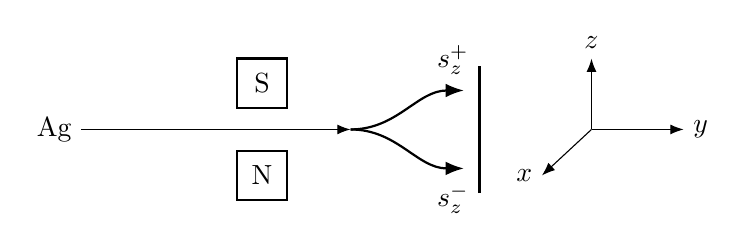
\begin{tikzpicture}[>=Latex,scale=.9]
 \draw[->] (-3.8,0)--(0,0); \node[left] at (-3.8,0){Ag};
 \draw[thick] (-1.6,.3) rectangle (-.9,1);\node at (-1.25,.65){S};
 \draw[thick] (-1.6,-1) rectangle (-.9,-.3);\node at (-1.25,-.65){N};
 \draw[->,thick] (0,0) to[out=0,in=180] (1.6,.55) node[above,xshift=-4pt,yshift=2pt] {$s_z^+$};
 \draw[->,thick] (0,0) to[out=0,in=180] (1.6,-.55) node[below,xshift=-4pt,yshift=-2pt] {$s_z^-$};
 \draw[thick] (1.82,-.9)--(1.82,.9);
 \draw[->] (3.4,0)--(3.4,1) node[above] {$z$};
 \draw[->] (3.4,0)--(4.7,0) node[right] {$y$};
 \draw[->] (3.4,0)--(2.7,-.65) node[left] {$x$};
\end{tikzpicture}
\end{center}
\subsection*{1) Results}
A heated beam of silver atoms splits into two beams after passing through an inhomogeneous magnetic field.
\subsection*{2) Analysis}
\begin{itemize}
\item The splitting is caused by interaction with the magnetic field and must therefore be due to the magnetic moment $\vect M$ of the atoms. The interaction potential is $V=-\vect M\cdot\vect B$.
\item The magnetic moment is proportional to the angular momentum $\vect J$: $\vect M\propto\vect J$.
\item The force on the atoms is
\begin{equation}
\vect F=-\vect\nabla V=M_z\frac{\partial B_z}{\partial z}\vect e_z\propto J_z\frac{\partial B_z}{\partial z}\vect e_z.
\end{equation}
\end{itemize}
The beam separates symmetrically into an upper and a lower component. This indicates that the angular momentum along the direction of the magnetic field (the $z$ direction) has only two components of equal magnitude and opposite directions.

If this angular momentum were produced by the rotation of the atoms themselves, the angular-momentum directions of the thermal atoms would be randomly distributed. After a large number of atoms passed through the magnetic field, their distribution on the screen would be symmetric and continuous, rather than consisting of two separated components. Thus the force does not originate from orbital angular momentum.

A silver atom has 47 electrons. Of these, 46 occupy filled shells with a spherically symmetric distribution and have no net angular momentum. The angular momentum of the silver atom is entirely due to the remaining valence electron. The separated two-component distribution shows that it is caused by the intrinsic angular momentum of the valence electron, denoted by $\vect s$. The component $s_z$ has only two values of equal magnitude and opposite direction, $s_z^+$ and $s_z^-$.
\subsection*{3) Quantum properties}
\begin{itemize}
\item Spin angular momentum exists as an intrinsic physical quantity (independent of space and time).
\item The values of spin angular momentum are discrete.
\item The magnetic field performs a measurement. A magnetic field in the $z$ direction measures the angular momentum in the $z$ direction.
\end{itemize}
\subsection*{4) Cascaded Stern--Gerlach experiments}
\begin{center}
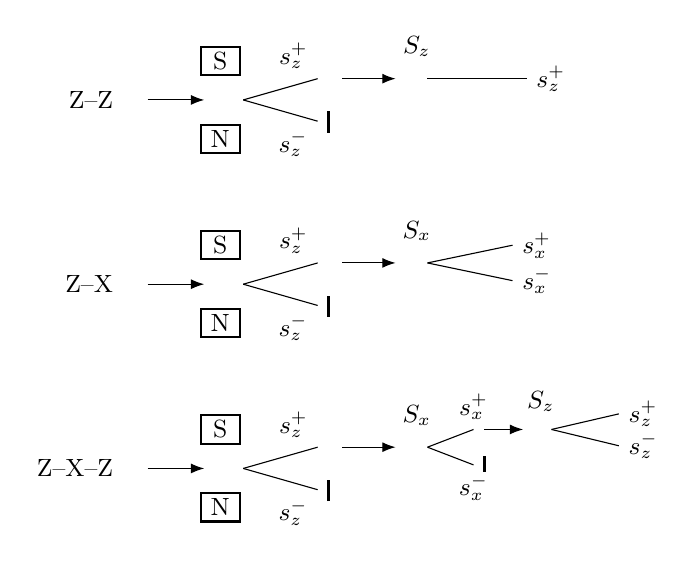
\begin{tikzpicture}[>=Latex,scale=.9, every node/.style={font=\small}]
\foreach \yy/\labs in {2.6/{Z--Z},0/{Z--X},-2.6/{Z--X--Z}}{
 \node[left] at (-4,\yy){\labs};
 \draw[->] (-3.65,\yy)--(-2.85,\yy);
 \draw[thick] (-2.9,\yy+.35) rectangle (-2.35,\yy+.75);\node at (-2.625,\yy+.55){S};
 \draw[thick] (-2.9,\yy-.75) rectangle (-2.35,\yy-.35);\node at (-2.625,\yy-.55){N};
 \draw (-2.3,\yy)--(-1.25,\yy+.3) node[above left] {$s_z^+$};
 \draw (-2.3,\yy)--(-1.25,\yy-.3) node[below left] {$s_z^-$};
 \draw[very thick] (-1.1,\yy-.46)--(-1.1,\yy-.16);
}
\draw[->] (-.9,2.9)--(-.15,2.9); \node at (.15,3.35){$S_z$};\draw (.3,2.9)--(1.7,2.9) node[right] {$s_z^+$};
\draw[->] (-.9,.3)--(-.15,.3);\node at (.15,.75){$S_x$};
\draw (.3,.3)--(1.5,.55) node[right] {$s_x^+$};\draw (.3,.3)--(1.5,.05) node[right] {$s_x^-$};
\draw[->] (-.9,-2.3)--(-.15,-2.3);\node at (.15,-1.85){$S_x$};
\draw (.3,-2.3)--(.95,-2.05) node[above] {$s_x^+$};\draw (.3,-2.3)--(.95,-2.55) node[below] {$s_x^-$};
\draw[very thick] (1.1,-2.65)--(1.1,-2.43);
\draw[->] (1.1,-2.05)--(1.65,-2.05);\node at (1.9,-1.65){$S_z$};
\draw (2.05,-2.05)--(3,-1.83) node[right] {$s_z^+$};\draw (2.05,-2.05)--(3,-2.28) node[right] {$s_z^-$};
\end{tikzpicture}
\par\smallskip Figure 1.
\end{center}
The incident atomic beam passes successively through two magnetic fields in the $z$ direction, as shown in the upper part of Fig.~1. Before the second magnetic field, $s_z$ has the definite value $s_z^+$. Therefore the force on the atoms in that field is definite, and $s_z$ still has the definite value $s_z^+$ after the second field.

Now let the incident atomic beam pass through two magnetic fields, in the $z$ and $x$ directions, as shown in the middle of Fig.~1. In the second magnetic field the atoms experience a force $\vect F\propto J_x(\partial B_x/\partial x)\vect e_x$. The beam splits after the second magnetic field, indicating that $s_x$ has two components $s_x^+$ and $s_x^-$ before that field, although $s_z$ has the definite value $s_z^+$.
\begin{itemize}\item Quantum property: when $s_z$ has a definite value, $s_x$ does not. $s_z$ and $s_x$ cannot have definite values simultaneously.\end{itemize}
Next, let the beam pass successively through three magnetic fields in the $z$, $x$, and $z$ directions, as shown in the lower part of Fig.~1. Finally one observes two components $s_z^+$ and $s_z^-$. Thus $s_z$ has two components before the third magnetic field, even though $s_x$ has the definite value $s_x^+$.
\begin{itemize}\item Quantum property: when $s_x$ has a definite value, $s_z$ likewise does not. $s_x$ and $s_z$ cannot have definite values simultaneously.\end{itemize}
\subsection*{5) Analogy with classical electromagnetic waves (matter particles and light waves)}
\begin{center}
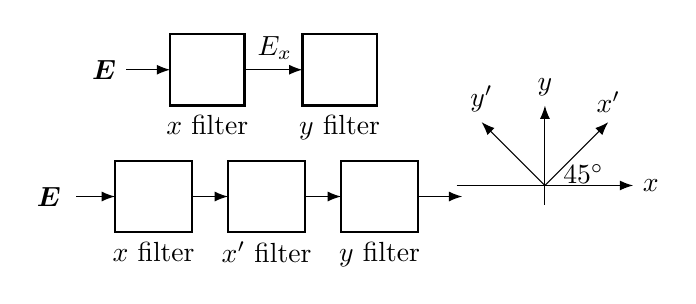
\begin{tikzpicture}[>=Latex,scale=.7]
\node at (-2,1){$\vect E$};\draw[->] (-1.6,1)--(-.8,1);
\draw[thick] (-.8,.35) rectangle (.55,1.65);\node[below] at (-.125,.35){$x$ filter};
\draw[->] (.55,1)--(1.6,1);\node[above] at (1.1,1){$E_x$};
\draw[thick] (1.6,.35) rectangle (2.95,1.65);\node[below] at (2.275,.35){$y$ filter};
\begin{scope}[yshift=-2.3cm]
\node at (-3,1){$\vect E$};\draw[->] (-2.5,1)--(-1.8,1);
\foreach \x/\lab in {-1.8/{$x$ filter},.25/{$x'$ filter},2.3/{$y$ filter}} {
 \draw[thick] (\x,.35) rectangle (\x+1.4,1.65);\node[below] at (\x+.7,.35){\lab};
}
\draw[->] (-.4,1)--(.25,1);\draw[->] (1.65,1)--(2.3,1);\draw[->] (3.7,1)--(4.5,1);
\end{scope}
\begin{scope}[shift={(6,-1.1)}]
\draw[->](-1.6,0)--(1.6,0) node[right]{$x$};\draw[->](0,-.35)--(0,1.45)node[above]{$y$};
\draw[->](0,0)--(1.15,1.15)node[above]{$x'$};\draw[->](0,0)--(-1.15,1.15)node[above]{$y'$};\node at (.7,.2){$45^\circ$};
\end{scope}
\end{tikzpicture}
\end{center}
An electromagnetic wave propagating along the $z$ direction disappears completely after passing successively through a filter that transmits only the $x$ component ($x$ filter) and a filter that transmits only the $y$ component ($y$ filter):
\begin{equation}\begin{aligned}
\vect E(\vect r,t)&=E_0(\vect e_x+\vect e_y)\cos(kz-\omega t),\\
\xrightarrow{x\text{ filter}}\quad &E_0\vect e_x\cos(kz-\omega t),\\
\xrightarrow{y\text{ filter}}\quad &0.
\end{aligned}\end{equation}
Place an $x'$ filter between the $x$ and $y$ filters, with $x'$ at $45^\circ$ to both $x$ and $y$. An electromagnetic wave in the $y$ direction can still be observed at the end:
\begin{equation}\begin{aligned}
\vect E(\vect r,t)&=E_0(\vect e_x+\vect e_y)\cos(kz-\omega t),\\
\xrightarrow{x\text{ filter}}\quad&E_0\vect e_x\cos(kz-\omega t)=\frac{E_0}{\sqrt2}(\vect e_{x'}-\vect e_{y'})\cos(kz-\omega t),\\
\xrightarrow{x'\text{ filter}}\quad&\frac{E_0}{\sqrt2}\vect e_{x'}\cos(kz-\omega t)=\frac{E_0}{2}(\vect e_x+\vect e_y)\cos(kz-\omega t),\\
\xrightarrow{y\text{ filter}}\quad&\frac{E_0}{2}\vect e_y\cos(kz-\omega t).
\end{aligned}\end{equation}
Similarity: $s_x,s_y,s_z$ and $E_{x'},E_{y'}$ can all be regarded as two-component vectors.

Difference: $\vect s$ is intrinsic angular momentum, a quantum-mechanical quantity; $\vect E$ is a spatially dependent mechanical quantity, a classical-mechanical quantity.
% SOURCE: original Chinese PDF, viewer pages 4--6.
\section{Linear Vector Spaces}
From the preceding section, the projection $s_n$ of the electron's spin angular momentum along any direction $n$ can take only two values. We may regard $s_n$ as a two-dimensional vector. To establish the mathematical description of quantum mechanics, we first discuss linear vector spaces.
\subsection*{1) Three-dimensional vector space}
\begin{center}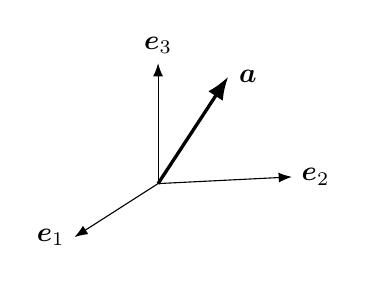
\begin{tikzpicture}[>=Latex,scale=.85]
\coordinate (O) at (0,0); \draw[->] (O)--(2.0,.1)node[right]{$\vect e_2$};\draw[->](O)--(-1.25,-.8)node[left]{$\vect e_1$};\draw[->](O)--(0,1.8)node[above]{$\vect e_3$};\draw[->,very thick](O)--(1.05,1.6)node[right]{$\vect a$};
\end{tikzpicture}\end{center}
Arbitrary vector: $\vect a$.

Basis vectors: $\vect e_n$, $n=1,2,3$.

Completeness of the basis:
\begin{equation}
\vect a=\sum_{n=1}^{3}a_n\vect e_n.
\end{equation}
Inner product:
\begin{equation}
\vect a\cdot\vect b=\sum_{n,m}a_nb_m\vect e_n\cdot\vect e_m.
\end{equation}
Squared norm of a vector: $\vect a\cdot\vect a\geq0$.

If the basis vectors are orthonormal, $\vect e_n\cdot\vect e_m=\delta_{nm}$, the inner product has the matrix form
\begin{equation}
\vect a\cdot\vect b=\sum_n a_nb_n=\widetilde a\,b,
\quad b=\begin{pmatrix}b_1\\b_2\\b_3\end{pmatrix},\quad
 a=\begin{pmatrix}a_1\\a_2\\a_3\end{pmatrix},\quad
 \widetilde a=(a_1,a_2,a_3),
\end{equation}
where $\widetilde a$ is the transpose of $a$.

Components (matrix elements) of a vector:
\begin{equation}
a_n=\vect e_n\cdot\vect a.
\end{equation}
The vector $\vect a$ is its abstract or general form. The matrix $a$ is the representation of $\vect a$ in a specific coordinate system (representation). Its matrix elements depend on the choice of basis vectors; for example, Cartesian and spherical coordinate systems give different representations.

Operations on a vector, such as translations and rotations (operators), give another vector in the same three-dimensional space: $\op T\vect a=\vect b$.
\subsection*{2) Hilbert space}
Extend the three-dimensional vector space to a complex vector space of arbitrary dimension:
\begin{equation}
\text{three dimensions}\longrightarrow\text{arbitrary finite, infinite, or continuous dimension},
\end{equation}
\begin{equation}
\text{constant vectors}\longrightarrow\text{complex-function vectors}.
\end{equation}
Use Dirac notation (a ket) to denote an arbitrary vector: $\ket a$.

For a complex vector, introduce the bra $\bra a$ to represent its complex-conjugate vector. The bra and ket are not independent; they are conjugate to each other:
\begin{equation}
\ket a\longleftrightarrow\bra a.
\end{equation}
A vector can be represented by either a ket $\ket a$ or a bra $\bra a$.

In a complex-function vector space, constants are generally complex, so
\begin{equation}
\alpha\ket a\longleftrightarrow\bra a\alpha^*.
\end{equation}
For an operation (operator) $\op T$ in the complex space,
\begin{equation}
\op T\ket a\longleftrightarrow\bra a\op T^\dagger.
\end{equation}
$\op T^\dagger$ is the left operator corresponding to the right operator $\op T$, called the Hermitian-conjugate operator. Note that
\begin{equation}
\op T\op F\ket a=\op T(\op F\ket a)
\longleftrightarrow \bra a\op F^\dagger\op T^\dagger.
\end{equation}
We now choose a particular representation, taking an $N$-dimensional discrete space as an example.

Basis vectors: $\ket n$, $n=1,2,\ldots$.

Expansion in a complete basis (concrete representation of a vector):
\begin{equation}
\ket a=\sum_n a_n\ket n,\qquad \bra a=\sum_n a_n^*\bra n.
\end{equation}
Inner product:
\begin{equation}
\braket a b=\sum_{n,m}a_n^*b_m\braket n m,
\end{equation}
which is a complex number.

Squared norm: $\braket a a\geq0$. (Only when $\ket a$ and $\bra a$ are defined as conjugates can the squared norm be guaranteed nonnegative.)

Normalized vector: defining $\ket{\widetilde a}=\ket a/\sqrt{\braket a a}$ gives $\braket{\widetilde a}{\widetilde a}=1$; the vector is said to be normalized.

Orthonormality of basis vectors: $\braket n m=\delta_{nm}$.

Matrix form of the inner product:
\begin{equation}
\braket a b=\sum_n a_n^*b_n=a^\dagger b,
\qquad b=\begin{pmatrix}b_1\\b_2\\\vdots\\b_N\end{pmatrix},\quad
 a=\begin{pmatrix}a_1\\a_2\\\vdots\\a_N\end{pmatrix},
\end{equation}
where the Hermitian conjugate (complex-conjugate transpose) of the column matrix $a$ is the row matrix
\begin{equation}
a^\dagger=(a_1^*,a_2^*,\ldots,a_N^*).
\end{equation}
Evidently,
\begin{equation}
\braket a b=\braket b a^*,\qquad
\mel a{\op T}b=\mel b{\op T^\dagger}a^*.
\end{equation}
Components (matrix elements) of a vector: multiplying $\ket a=\sum_n a_n\ket n$ from the left by $\bra m$ gives
\begin{equation}
a_m=\braket m a.
\end{equation}
Completeness of the basis:
\begin{equation}
\ket a=\sum_n a_n\ket n=\sum_n\ket n\braket n a
=\left(\sum_n\ket n\bra n\right)\ket a.
\end{equation}
Because $\ket a$ is arbitrary,
\begin{equation}
\boxed{\sum_n\ket n\bra n=\mathbf 1},
\end{equation}
which is the completeness relation for the basis.

\paragraph{Representation of an operator (matrix form).}
Let $\ket b=\op F\ket a$. Then
\begin{equation}
\braket m b=\mel m{\op F}a
=\sum_n\mel m{\op F}n\braket n a,
\qquad F_{mn}=\mel m{\op F}n,
\end{equation}
and therefore
\begin{equation}
b_m=\sum_n F_{mn}a_n.
\end{equation}
In matrix form, $b=Fa$. The matrix $F$ represents the operator $\op F$; it is a square matrix with elements $F_{mn}$.
\paragraph{Representation of the Hermitian-conjugate operator (left operator).}
From $\bra b=\bra a\op F^\dagger$,
\begin{equation}
\braket b m=\mel a{\op F^\dagger}m
=\sum_n\braket a n\mel n{\op F^\dagger}m,
\end{equation}
so
\begin{equation}
b_m^*=\sum_n (F^\dagger)_{nm}a_n^*,\qquad
b_m=\sum_n[(F^\dagger)_{nm}]^*a_n.
\end{equation}
Comparison yields
\begin{equation}
[(F^\dagger)_{nm}]^*=F_{mn},\qquad
(F^\dagger)_{nm}=F_{mn}^*,\qquad
F^\dagger=(\widetilde F)^*.
\end{equation}
Thus $F^\dagger$ is the Hermitian-conjugate matrix of $F$.
\paragraph{Outer product.}
The outer product is $\ket a\bra b$.

Its representation is a square matrix ($a$ is a column matrix and $b^\dagger$ a row matrix), so the outer product is an operator. In fact,
\begin{equation}
(\ket a\bra b)\ket c=\ket a(\braket b c),
\end{equation}
showing that $\ket a\bra b$ maps $\ket c$ to another vector parallel to $\ket a$. Hence $\ket a\bra b$ is indeed an operator. Its representation is a square matrix with elements
\begin{equation}
(\ket a\bra b)_{mn}=\mel m{\ket a\bra b}n
=\braket m a\braket b n=a_mb_n^*.
\end{equation}
% SOURCE: original Chinese PDF, viewer pages 7--9.
\section{Eigenvalues and Eigenvectors of Operators (Matrices)}
\subsection*{1) Eigenvalues and eigenstates of a general operator}
The eigenvalue equation of an operator is
\begin{equation}
\op T\ket a=\lambda\ket a,
\end{equation}
where $\lambda$ is called an eigenvalue of $\op T$ and $\ket a$ is called an eigenvector of $\op T$.

In matrix form (prove this yourself using the completeness relation),
\begin{equation}
Ta=\lambda a,\qquad (T-\lambda I)a=0.
\end{equation}
The condition for a nonzero eigenvector $a\ne0$ is
\begin{equation}
\det(T-\lambda I)=0.
\end{equation}
This is the secular equation in an $N$-dimensional space:
\begin{equation}
\begin{vmatrix}
T_{11}-\lambda&T_{12}&\cdots&T_{1N}\\
T_{21}&T_{22}-\lambda&\cdots&T_{2N}\\
\vdots&\vdots&\ddots&\vdots\\
T_{N1}&T_{N2}&\cdots&T_{NN}-\lambda
\end{vmatrix}=0.
\end{equation}
One thereby obtains $N$ eigenvalues $\lambda_i$ ($i=1,2,\ldots,N$). Substituting each into
\begin{equation}
(T-\lambda_i I)a=0
\end{equation}
gives the corresponding eigenvector $a$.

\textbf{Example.} Find the eigenvalues and eigenvectors of
\begin{equation}
T=\begin{pmatrix}1&0\\0&-1\end{pmatrix}.
\end{equation}
The secular equation is
\begin{equation}
\begin{vmatrix}1-\lambda&0\\0&-1-\lambda\end{vmatrix}=0,
\quad\text{i.e.,}\quad \lambda^2-1=0,
\end{equation}
and the eigenvalues are $\lambda_\pm=\pm1$.

Let $a=(a_1,a_2)^{\mathsf T}$. For $\lambda=1$,
\begin{equation}
\begin{pmatrix}0&0\\0&-2\end{pmatrix}
\begin{pmatrix}a_1\\a_2\end{pmatrix}=0.
\end{equation}
The normalized eigenvector is $a=(1,0)^{\mathsf T}$. Similarly, taking $\lambda=-1$ gives $a=(0,1)^{\mathsf T}$.
\subsection*{2) Hermitian operators}
If $\op T^\dagger=\op T$, or $T^\dagger=T$, the operator $\op T$ is called Hermitian and $T$ is called a Hermitian matrix.

We discuss the following properties of Hermitian operators.
\paragraph{a) Conjugate symmetry.}
\begin{equation}
\mel a{\op T}b=\mel b{\op T^\dagger}a^*=\mel b{\op T}a^*.
\end{equation}
In particular,
\begin{equation}
\mel a{\op T}a=\mel a{\op T}a^*,
\end{equation}
which shows that the expectation value $\mel a{\op T}a$ of a Hermitian operator is real.

For an anti-Hermitian operator, $\op T^\dagger=-\op T$ and
\begin{equation}
\mel a{\op T}a=-\mel a{\op T}a^*,
\end{equation}
so its expectation value is purely imaginary.
\paragraph{b) Reality of eigenvalues and orthogonality.}
Suppose
\begin{equation}
\op T\ket i=\lambda_i\ket i,\qquad \op T\ket j=\lambda_j\ket j.
\end{equation}
From
\begin{equation}
\mel j{\op T}i=\lambda_i\braket j i
\end{equation}
and
\begin{equation}
\bra j\op T=\bra j\lambda_j^*,\qquad
\mel j{\op T}i=\lambda_j^*\braket j i,
\end{equation}
we obtain
\begin{equation}
(\lambda_i-\lambda_j^*)\braket j i=0.
\end{equation}
For $j=i$ and $\braket i i\ne0$, $\lambda_i=\lambda_i^*$: the eigenvalues of a Hermitian operator are real.

For $j\ne i$, if $\lambda_i-\lambda_j\ne0$, then $\braket j i=0$. Thus eigenstates corresponding to different eigenvalues of a Hermitian operator are orthogonal. Since they can always be normalized, the orthonormality condition is
\begin{equation}
\braket i j=\delta_{ij}.
\end{equation}
\textbf{Question:} Are eigenstates corresponding to the same eigenvalue orthogonal?
\paragraph{c) Orthogonalization by linear superposition (Schmidt orthogonalization).}
Suppose several eigenstates correspond to the same eigenvalue, i.e., there is degeneracy. For example, for a $g$-fold degenerate eigenvalue ($g\ge2$),
\begin{equation}
\op T\ket{i,j}=\lambda_i\ket{i,j},\qquad j=1,\ldots,g.
\end{equation}
Are these $g$ eigenvectors orthogonal?

Redefine $g$ new states:
\begin{equation}
\ket{i,n}=\sum_{j=1}^g C_{nj}\ket{i,j},\qquad n=1,2,\ldots,g.
\end{equation}
Since
\begin{equation}
\op T\ket{i,n}=\sum_{j=1}^g C_{nj}\op T\ket{i,j}
=\lambda_i\sum_{j=1}^g C_{nj}\ket{i,j}=\lambda_i\ket{i,n},
\end{equation}
each $\ket{i,n}$ is still an eigenstate of $\op T$ with eigenvalue $\lambda_i$. Hence it suffices to show that the $\ket{i,n}$ can be made orthonormal.

Can one choose the coefficients $C_{nj}$ so that these $g$ new states satisfy
\begin{equation}
\braket{i,m}{i,n}=\delta_{mn}\;?
\end{equation}
There are $g$ normalization equations and $(g^2-g)/2$ orthogonality equations, making $g(g+1)/2$ independent equations, fewer than the $g^2$ coefficients $C_{nj}$. Thus there are various choices of coefficients satisfying the orthonormality conditions, so that the new states $\ket{i,n}$ are orthonormal:
\begin{equation}
\braket{i,m}{j,n}=\delta_{ij}\delta_{mn}.
\end{equation}
Here $\delta_{ij}$ follows from orthonormality of eigenstates belonging to different eigenvalues, while $\delta_{mn}$ follows from orthogonalization by linear superposition.

\textbf{Conclusion:} Eigenstates of a Hermitian operator can be chosen orthonormal, whether the eigenvalues are degenerate or nondegenerate.
\paragraph{d) Completeness.}
It can be shown that eigenvectors of a Hermitian operator satisfy
\begin{equation}
\sum_i\ket i\bra i=\mathbf1.
\end{equation}
Hence the eigenvectors of a Hermitian operator can form a set of orthonormal basis vectors of a Hilbert space, i.e., a linear vector space or a representation.
% SOURCE: original Chinese PDF, viewer pages 9--16.
\section{Measurement}
We discuss the connection between quantum mechanics and Hilbert space.
\subsection*{1) Measurement of a single physical quantity}
In the Stern--Gerlach experiment, $s_z$ has no definite value before the magnetic field (if it did, only one beam of silver atoms would emerge). It has a definite value only after the field: one beam has $s_z^+$, and the other has $s_z^-$. Therefore the values of quantum-mechanical quantities are closely related to the state of the system. A physical quantity has no definite value in a general state; it has a definite value only in certain particular states.

\textbf{Postulate of quantum mechanics:} Physical quantities of a quantum-mechanical system are represented by Hermitian operators in a linear vector space, and states are represented by vectors. Because the eigenstates of a Hermitian operator are complete, the eigenstates of any physical quantity can form a linear vector space, or a representation.

The eigenvalue equation of $\op F$ is
\begin{equation}
\op F\ket n=f_n\ket n.
\end{equation}
In the $F$ representation, the basis vectors are $\ket n$. An arbitrary state is
\begin{equation}
\ket a=\sum_n\ket n\braket n a.
\end{equation}
The coefficient $\braket n a$ is the concrete representation of $\ket a$ in the $F$ representation.

\textbf{Postulate of quantum mechanics:} The physical quantity $\op F$ has a definite value, namely the eigenvalue $f_n$, only in its eigenstate $\ket n$. In an arbitrary state $\ket a$, $\op F$ has no definite value, but has a definite average value
\begin{equation}
\langle F\rangle\equiv\mel a{\op F}a.
\end{equation}
(The eigenvalues and expectation values of Hermitian operators are real. This is why physical quantities are represented by Hermitian operators.)
\begin{equation}\begin{aligned}
\langle F\rangle
&\equiv\mel a{\op F}a
=\sum_{n,m}\braket a n\mel n{\op F}m\braket m a\\
&=\sum_{n,m}\braket a n f_m\delta_{nm}\braket m a
=\sum_n\braket a n\braket n a f_n
=\sum_n|\braket n a|^2f_n.
\end{aligned}\end{equation}
Thus the probability that $\op F$ takes the value $f_n$ is $|\braket n a|^2$. The quantity $\braket n a$ is a probability amplitude, and $|\braket n a|^2$ is the probability for state $\ket a$ to contain state $\ket n$.

In a general state, the value of a physical quantity is uncertain, but its probabilities and expectation value are definite.

In the eigenbasis of $\op F$, the matrix elements are
\begin{equation}
F_{mn}=\mel m{\op F}n=f_n\braket m n=f_n\delta_{mn}.
\end{equation}
Thus a physical quantity is represented by a diagonal matrix in its own representation, and the diagonal elements are its eigenvalues.

We now discuss measurement and collapse of the state.

Before the magnetic field in the Stern--Gerlach experiment, $s_z$ of an Ag atom has no definite value; after passing through the field it has a definite value. Applying the magnetic field can be regarded as measuring the spin. Once measured, it has a definite value.

When $\op F$ is measured in an arbitrary state $\ket a$, the system collapses into an eigenstate of $\op F$, so $\op F$ has a definite value. Which eigenstate does it collapse into? The probability for state $\ket a$ to contain state $\ket n$ is $|\braket n a|^2$. Therefore the probability of collapse into $\ket n$, i.e., of obtaining the measurement value $f_n$, is $|\braket n a|^2$.

Measurement allows the particle nature of the system to become manifest; one may also say that measurement produces a particle.

\textbf{Question:} Measure $\op F$ in state $\ket a$ and obtain $f_n$. If $\op F$ is measured again immediately, what value will be obtained?

First measurement: $\ket a\longrightarrow\ket n$.

At the second measurement, the system is already in the eigenstate $\ket n$ of $\op F$; the result is still $f_n$. This explains why an Ag atom in the Stern--Gerlach experiment still has spin $s_z^+$ after passing through two magnetic fields in the $z$ direction.
\subsection*{2) Spin matrices}
From the Stern--Gerlach experiment, the electron has spin $1/2$, and the spin operator $\vect{\op s}\cdot\vect e_n=\op s_n$ along any direction $\vect e_n$ takes the values $\pm\hbar/2$. Its eigenvalue equation is
\begin{equation}
\op s_n\ket{s_n^\pm}=\pm\frac\hbar2\ket{s_n^\pm}.
\end{equation}
In the representation formed by the eigenstates of $\op s_z$ (the $s_z$ representation), $s_z$ is a diagonal matrix whose diagonal entries are $\pm\hbar/2$:
\begin{equation}
s_z=\frac\hbar2\begin{pmatrix}1&0\\0&-1\end{pmatrix}.
\end{equation}
Solving
\begin{equation}
s_z\begin{pmatrix}a\\b\end{pmatrix}=\pm\frac\hbar2\begin{pmatrix}a\\b\end{pmatrix}
\end{equation}
gives the normalized eigenstates
\begin{equation}
\ket{s_z^+}=\begin{pmatrix}1\\0\end{pmatrix},\qquad
\ket{s_z^-}=\begin{pmatrix}0\\1\end{pmatrix}.
\end{equation}
We now find the matrices for $\op s_x$ and $\op s_y$ in the $s_z$ representation. From the completeness of the eigenstates of $\op s_z$,
\begin{equation}
\ket{s_x^+}=\sum_{i=\pm}\ket{s_z^i}\braket{s_z^i}{s_x^+}
=\braket{s_z^+}{s_x^+}\ket{s_z^+}
+\braket{s_z^-}{s_x^+}\ket{s_z^-}.
\end{equation}
The cascaded Stern--Gerlach experiment shows that a state with a definite $s_x$ value, after passing through a $z$-directed magnetic field (a measurement device for $s_z$), separates into two beams of equal intensity, with equal probabilities for $s_z^+$ and $s_z^-$:
\begin{equation}
|\braket{s_z^+}{s_x^+}|=|\braket{s_z^-}{s_x^+}|=\frac1{\sqrt2}.
\end{equation}
Consequently,
\begin{equation}
\ket{s_x^+}=\frac1{\sqrt2}\ket{s_z^+}+\frac1{\sqrt2}e^{\ii\delta_1}\ket{s_z^-}.
\end{equation}
Through normalization, the phase factors have been collected into $\delta_1$.

Using the orthonormality of $\ket{s_x^\pm}$,
$\braket{s_x^i}{s_x^j}=\delta_{ij}$, we obtain
\begin{equation}
\ket{s_x^-}=\frac1{\sqrt2}\ket{s_z^+}-\frac1{\sqrt2}e^{\ii\delta_1}\ket{s_z^-}.
\end{equation}
Equivalently,
\begin{equation}
\begin{cases}
\displaystyle\ket{s_z^+}=\frac1{\sqrt2}(\ket{s_x^+}+\ket{s_x^-}),\\[5pt]
\displaystyle\ket{s_z^-}=\frac1{\sqrt2}e^{-\ii\delta_1}(\ket{s_x^+}-\ket{s_x^-}).
\end{cases}
\end{equation}
Substituting into the matrix elements of $\op s_x$ gives
\begin{equation}
\mel{s_z^+}{\op s_x}{s_z^+}=0,\quad
\mel{s_z^+}{\op s_x}{s_z^-}=\frac\hbar2e^{-\ii\delta_1},\quad
\mel{s_z^-}{\op s_x}{s_z^+}=\frac\hbar2e^{\ii\delta_1},\quad
\mel{s_z^-}{\op s_x}{s_z^-}=0.
\end{equation}
Thus
\begin{equation}
s_x=\frac\hbar2\begin{pmatrix}0&e^{-\ii\delta_1}\\e^{\ii\delta_1}&0\end{pmatrix}.
\end{equation}
Similarly,
\begin{equation}
\ket{s_y^\pm}=\frac1{\sqrt2}\ket{s_z^+}\pm\frac1{\sqrt2}e^{\ii\delta_2}\ket{s_z^-},\qquad
s_y=\frac\hbar2\begin{pmatrix}0&e^{-\ii\delta_2}\\e^{\ii\delta_2}&0\end{pmatrix}.
\end{equation}
Now consider the values of $\delta_1,\delta_2$. A state with a definite $s_x$ value, after passing through a magnetic field in the $y$ direction (a measurement device for $s_y$), splits into two equally intense beams corresponding to $s_y^+$ and $s_y^-$:
\begin{equation}
|\braket{s_y^\pm}{s_x^+}|=\frac1{\sqrt2}.
\end{equation}
That is,
\begin{equation}
\frac12\left|1\pm e^{\ii(\delta_1-\delta_2)}\right|=\frac1{\sqrt2}.
\end{equation}
Hence
\begin{equation}
\delta_1-\delta_2=\pm\frac\pi2.
\end{equation}
Choosing $\delta_1=0$ and $\delta_2=\pi/2$ yields
\begin{equation}
s_x=\frac\hbar2\begin{pmatrix}0&1\\1&0\end{pmatrix},\qquad
s_y=\frac\hbar2\begin{pmatrix}0&-\ii\\\ii&0\end{pmatrix}.
\end{equation}
For $s_x,s_y,s_z$, one can show that
\begin{equation}
 [s_i,s_j]=\ii\epsilon_{ijk}\hbar s_k,\qquad
\{s_i,s_j\}=\frac{\hbar^2}{2}\delta_{ij},
\end{equation}
where
\begin{equation}
[A,B]=AB-BA,\qquad\{A,B\}=AB+BA.
\end{equation}
Define
\begin{equation}
s^2=\sum_i s_i^2=\frac{3}{4}\hbar^2\begin{pmatrix}1&0\\0&1\end{pmatrix}.
\end{equation}
Because $s^2$ is proportional to the identity matrix, every state is its eigenstate, and it has the definite value $3\hbar^2/4$ in every state. Clearly, $\op{s^2}$ commutes with every physical quantity $\op F$ and may be regarded as a classical quantity.
\subsection*{3) Conditions for simultaneous measurement of several physical quantities}
Can two physical quantities $\op A$ and $\op B$ be measured simultaneously?

\textbf{Theorem.} If $\op A$ and $\op B$ have a complete set of common eigenstates, then $\op A$ and $\op B$ commute.

\textbf{Proof.} Let the complete common eigenstates be $\ket n$, with
\begin{equation}
\op A\ket n=a_n\ket n,\qquad \op B\ket n=b_n\ket n.
\end{equation}
In the representation formed by $\ket n$, an arbitrary state is
\begin{equation}
\ket\psi=\sum_n\ket n\braket n\psi.
\end{equation}
Then
\begin{equation}\begin{aligned}
(\op A\op B-\op B\op A)\ket\psi
&=\sum_n(\op A\op B-\op B\op A)\ket n\braket n\psi\\
&=\sum_n(\op A b_n-\op B a_n)\ket n\braket n\psi\\
&=\sum_n(a_nb_n-b_na_n)\ket n\braket n\psi=0.
\end{aligned}\end{equation}
Since $\ket\psi$ is arbitrary, $[\op A,\op B]=0$.

\textbf{Converse theorem.} If $\op A$ and $\op B$ commute, then they have a complete set of common eigenstates.

\textbf{Proof.} Let $\ket n$ be an eigenstate of $\op A$:
\begin{equation}
\op A\ket n=a_n\ket n.
\end{equation}
From $[\op A,\op B]=0$,
\begin{equation}
\op A\op B\ket n=\op B\op A\ket n=a_n\op B\ket n.
\end{equation}
Thus $\op B\ket n$ is also an eigenstate of $\op A$ with eigenvalue $a_n$. If $\op A$ is nondegenerate, $\op B\ket n$ and $\ket n$ are the same state up to a constant:
\begin{equation}
\op B\ket n=b_n\ket n.
\end{equation}
Therefore $\ket n$ is also an eigenstate of $\op B$, and $\op A$ and $\op B$ have a complete common eigenbasis.

If $\op A$ is degenerate, one can use the Schmidt method to prove the same result (exercise).

\textbf{Conclusion.} When several physical quantities commute, they can have common eigenstates. In those common eigenstates, all these quantities have definite values, and they can be measured simultaneously.

Note that $[\op A,\op B]=0$ and $[\op B,\op C]=0$ mean that $A,B$ can have definite values simultaneously and that $B,C$ can have definite values simultaneously. However, $A,C$ need not have definite values simultaneously.

When $\op A$ and $\op B$ do not commute, they cannot have a complete set of common eigenstates and cannot always be measured simultaneously. They may, however, be simultaneously measurable in a subspace. For example, for orbital angular momentum,
\begin{equation}
[\op{\vect L}^{\,2},\op L_x]=0,\qquad [\op{\vect L}^{\,2},\op L_y]=0,\qquad [\op L_x,\op L_y]\ne0.
\end{equation}
Thus $L^2,L_x$ can have definite values simultaneously, and $L^2,L_y$ can have definite values simultaneously, while $L_x,L_y$ cannot generally have definite values simultaneously. In the state with $L=0$, however, $L_x,L_y$ are simultaneously definite, with $L_x=L_y=0$.
\subsection*{4) Complete set of physical quantities}
When eigenvalues and eigenstates of a physical quantity are degenerate,
\begin{equation}
\op F\ket{i,j}=f_i\ket{i,j},\qquad j=1,\ldots,g,
\end{equation}
Schmidt orthogonalization can be used mathematically to obtain orthonormal eigenstates. In physics, however, one generally introduces a complete set of physical quantities to achieve orthonormality.

That several eigenstates share one eigenvalue indicates that this physical quantity is insufficient to characterize the states completely; another physical quantity is needed to distinguish them. Introduce $\op T$ and require that the eigenstates of $\op F$ also be eigenstates of $\op T$:
\begin{equation}
\op F\ket{i,j}=f_i\ket{i,j},\qquad
  \op T\ket{i,j}=t_j\ket{i,j}.
\end{equation}
For the set $\{\op F,\op T\}$, if the pair of eigenvalues $\{f_i,t_j\}$ corresponds one-to-one to the eigenstate $\ket{i,j}$, there is no degeneracy, and the orthonormality condition is
\begin{equation}
\braket{i,j}{i',j'}=\delta_{ii'}\delta_{jj'}.
\end{equation}
\subsection*{5) Cascaded measurements}
For three physical quantities $\op A,\op B,\op C$, consider the following two measurement procedures.

\textbf{First procedure:}
\begin{center}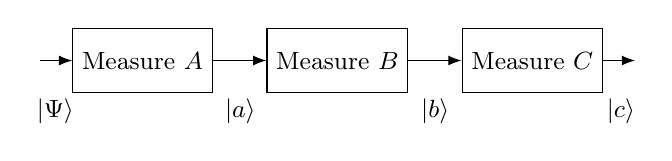
\begin{tikzpicture}[>=Latex,scale=.9,
 every node/.style={font=\small}]
 \node[draw,minimum width=1.75cm,minimum height=.82cm] (a) at (0,0) {Measure $A$};
 \node[draw,minimum width=1.75cm,minimum height=.82cm] (b) at (2.75,0) {Measure $B$};
 \node[draw,minimum width=1.75cm,minimum height=.82cm] (c) at (5.5,0) {Measure $C$};
 \draw[->] (-1.45,0)--(a.west);
 \draw[->] (a.east)--(b.west);
 \draw[->] (b.east)--(c.west);
 \draw[->] (c.east)--(6.95,0);
 \node[below] at (-1.23,-.40) {$\ket\Psi$};
 \node[below] at (1.38,-.40) {$\ket a$};
 \node[below] at (4.13,-.40) {$\ket b$};
 \node[below] at (6.75,-.40) {$\ket c$};
\end{tikzpicture}\end{center}
The state sequence is $\ket\Psi\rightarrow\ket a\rightarrow\ket b\rightarrow\ket c$; the values of the physical quantities are initially indefinite and then are $a,b,c$ after their respective measurements.

After three measurements, the probability for $\op C$ to take the value $c$ is
\begin{equation}
P(c)=\sum_{a,b}|\braket a\Psi|^2\,|\braket b a|^2\,|\braket c b|^2.
\end{equation}
Here $|\braket a\Psi|^2$ is the probability of collapse from $\ket\Psi$ to $\ket a$; $|\braket b a|^2$ is the probability from $\ket a$ to $\ket b$; and $|\braket c b|^2$ is the probability from $\ket b$ to $\ket c$.

\textbf{Second procedure:}
\begin{center}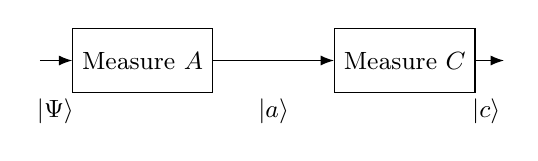
\begin{tikzpicture}[>=Latex,scale=.9,every node/.style={font=\small}]
 \node[draw,minimum width=1.75cm,minimum height=.82cm] (a) at (0,0) {Measure $A$};
 \node[draw,minimum width=1.75cm,minimum height=.82cm] (c) at (3.7,0) {Measure $C$};
 \draw[->] (-1.45,0)--(a.west);
 \draw[->] (a.east)--(c.west);
 \draw[->] (c.east)--(5.1,0);
 \node[below] at (-1.23,-.40) {$\ket\Psi$};
 \node[below] at (1.85,-.40) {$\ket a$};
 \node[below] at (4.85,-.40) {$\ket c$};
\end{tikzpicture}\end{center}
After two measurements, the probability for $\op C$ to take the value $c$ is
\begin{equation}
P'(c)=\sum_a |\braket a\Psi|^2\,|\braket c a|^2.
\end{equation}
Clearly, in general,
\begin{equation}
P(c)\ne P'(c).
\end{equation}
However, if $[\op A,\op B]=0$, $\op A$ and $\op B$ have common eigenstates $\ket n$, which replace $\ket a$ and $\ket b$:
\begin{equation}
P(c)=\sum_n|\braket n\Psi|^2\,|\braket c n|^2=P'(c).
\end{equation}
Or if $[\op B,\op C]=0$, $\op B$ and $\op C$ have common eigenstates $\ket m$, which replace $\ket b$ and $\ket c$:
\begin{equation}
P(c)=\sum_a|\braket a\Psi|^2\,|\braket m a|^2=P'(c).
\end{equation}
\textbf{Conclusion.} Since physical quantities have definite values only in their eigenstates, the order of measurements changes the final measurement results.
\subsection*{6) Uncertainty relation}
If $[\op A,\op B]\ne0$, the physical quantities $\op A,\op B$ cannot have definite values simultaneously. How large are their uncertainties?

In an arbitrary state $\ket\psi$, $\op A$ has only a definite expectation value $\langle\op A\rangle\equiv\mel\psi{\op A}\psi$ and a distribution $P(A)$.
\begin{center}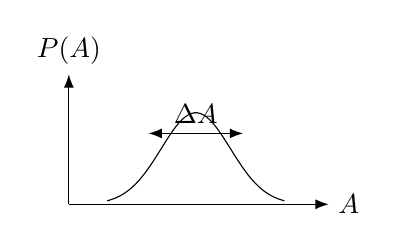
\begin{tikzpicture}[>=Latex,scale=.75]
\draw[->](0,0)--(4.4,0)node[right]{$A$};\draw[->](0,0)--(0,2.2)node[above]{$P(A)$};
\draw[domain=.65:3.65,samples=60,smooth,variable=\x] plot ({\x},{1.55*exp(-1.45*(\x-2.15)^2)});
\draw[<->] (1.35,1.2)--(2.95,1.2)node[midway,above]{$\Delta A$};
\end{tikzpicture}\end{center}
The uncertainty is represented by the variance:
\begin{equation}
\langle(\Delta\op A)^2\rangle\equiv
\mel\psi{(\op A-\langle\op A\rangle)^2}\psi\ge0.
\end{equation}
If $\ket\psi$ is an eigenstate of $\op A$, the expectation value equals its eigenvalue, the variance is zero, and the distribution is a delta function.
\begin{center}\begin{tikzpicture}[>=Latex,scale=.75]
\draw[->](0,0)--(4.4,0)node[right]{$A$};\draw[->](0,0)--(0,2.2)node[above]{$P(A)$};\draw[very thick](2.15,0)--(2.15,1.9);\node[below]at(2.15,0){$a$};
\end{tikzpicture}\end{center}
Define the uncertainty between $\op A$ and $\op B$ using the product of variances $\langle(\Delta\op A)^2\rangle\langle(\Delta\op B)^2\rangle$. How can we estimate it?

For arbitrary states $\ket\alpha,\ket\beta$ and arbitrary complex number $\lambda$, the norm of the linear-combination state is nonnegative:
\begin{equation}
(\bra\alpha+\lambda^*\bra\beta)(\ket\alpha+\lambda\ket\beta)\ge0.
\end{equation}
Choosing
\begin{equation}
\lambda=-\frac{\braket\beta\alpha}{\braket\beta\beta}
\end{equation}
gives the Schwarz inequality,
\begin{equation}
\braket\alpha\alpha\,\braket\beta\beta\ge |\braket\alpha\beta|^2.
\end{equation}
Set
\begin{equation}
\ket\alpha=\Delta\op A\ket\Psi,\qquad
\ket\beta=\Delta\op B\ket\Psi,\qquad
\Delta\op A=\op A-\langle\op A\rangle,\quad
\Delta\op B=\op B-\langle\op B\rangle.
\end{equation}
Then
\begin{equation}
\langle(\Delta\op A)^2\rangle\langle(\Delta\op B)^2\rangle
\ge |\langle\Delta\op A\Delta\op B\rangle|^2.
\end{equation}
Since
\begin{equation}\begin{aligned}
|\langle\Delta\op A\Delta\op B\rangle|^2
&=(\operatorname{Re}\langle\Delta\op A\Delta\op B\rangle)^2
 +(\operatorname{Im}\langle\Delta\op A\Delta\op B\rangle)^2\\
&\ge(\operatorname{Im}\langle\Delta\op A\Delta\op B\rangle)^2\\
&=\left[\frac1{2\ii}\left(\langle\Delta\op A\Delta\op B\rangle
-\langle\Delta\op B\Delta\op A\rangle\right)\right]^2,
\end{aligned}\end{equation}
we obtain
\begin{equation}
\langle(\Delta\op A)^2\rangle\langle(\Delta\op B)^2\rangle
\ge \left[\frac1{2\ii}\left(\langle\Delta\op A\Delta\op B\rangle
-\langle\Delta\op B\Delta\op A\rangle\right)\right]^2.
\end{equation}
Equality requires equality in the Schwarz inequality and a vanishing real part of $\langle\Delta\op A\Delta\op B\rangle$.

From
\begin{equation}\begin{aligned}
\langle\Delta\op A\Delta\op B\rangle
&=\mel\psi{(\op A-\langle\op A\rangle)(\op B-\langle\op B\rangle)}\psi
=\langle\op A\op B\rangle-\langle\op A\rangle\langle\op B\rangle,\\
\langle\Delta\op B\Delta\op A\rangle
&=\mel\psi{(\op B-\langle\op B\rangle)(\op A-\langle\op A\rangle)}\psi
=\langle\op B\op A\rangle-\langle\op B\rangle\langle\op A\rangle,
\end{aligned}\end{equation}
it follows that
\begin{equation}
\boxed{\langle(\Delta\op A)^2\rangle\langle(\Delta\op B)^2\rangle
\ge \left(\frac1{2\ii}\langle[\op A,\op B]\rangle\right)^2.}
\end{equation}
This shows that the uncertainties of two physical quantities are controlled by their commutation relation and the state $\ket\psi$.
% SOURCE: original Chinese PDF, viewer pages 16--18.
\section{Transformation of Representations}
Selecting a suitable representation can simplify a calculation. The transformation between basis vectors of different representations is called a transformation of representation.

Consider two representations:
\begin{equation}
\begin{array}{ll}
F\text{ representation:}&\text{basis }\ket i,\quad \op F\ket i=f_i\ket i,\\
G\text{ representation:}&\text{basis }\ket m,\quad \op G\ket m=g_m\ket m.
\end{array}
\end{equation}
We have
\begin{equation}
\ket m=\sum_i\ket i\braket i m=\sum_i S_{im}\ket i.
\end{equation}
The transformation matrix $S$ is defined by
\begin{equation}
S_{im}=\braket i m.
\end{equation}
It represents the basis vectors of the $M$ representation in the $I$ representation.
\subsection*{1) Transformation of an arbitrary vector}
In the $I$ representation,
\begin{equation}
\ket a=\sum_i\ket i\braket i a.
\end{equation}
The coefficient $\braket i a$ is the component of $\ket a$ along $\ket i$, or its representation in the $I$ basis.

In the $M$ representation,
\begin{equation}
\ket a=\sum_m\ket m\braket m a.
\end{equation}
The coefficient $\braket m a$ is the component along $\ket m$, or the representation of $\ket a$ in the $M$ basis.

Using completeness,
\begin{equation}
\braket m a=\sum_i\braket m i\braket i a
=\sum_i S_{im}^*\braket i a
=\sum_i S_{mi}^\dagger\braket i a.
\end{equation}
In matrix form,
\begin{equation}
\boxed{a_G=S^\dagger a_F.}
\end{equation}
\subsection*{2) Transformation of an arbitrary operator}
In the $I$ representation,
\begin{equation}
(A_F)_{ij}=\mel i{\op A}j.
\end{equation}
In the $M$ representation,
\begin{equation}\begin{aligned}
(A_G)_{mn}=\mel m{\op A}n
&=\sum_{ij}\braket m i\mel i{\op A}j\braket j n\\
&=\sum_{ij}S_{im}^*(A_F)_{ij}S_{jn}
=\sum_{ij}(S^\dagger)_{mi}(A_F)_{ij}S_{jn}.
\end{aligned}\end{equation}
In matrix form,
\begin{equation}
\boxed{A_G=S^\dagger A_F S.}
\end{equation}
\subsection*{3) The representation-transformation matrix is unitary}
\begin{equation}
(SS^\dagger)_{ij}=\sum_m S_{im}(S^\dagger)_{mj}
=\sum_m S_{im}S_{jm}^*
=\sum_m\braket i m\braket m j
=\braket i j=\delta_{ij}.
\end{equation}
Therefore $SS^\dagger=\mathbf1$. Similarly, $S^\dagger S=\mathbf1$, and hence
\begin{equation}
\boxed{S^\dagger=S^{-1}.}
\end{equation}
A representation-transformation matrix is unitary.

Note that $S$ is not necessarily Hermitian: $S^\dagger\ne S$.
\subsection*{4) Transformation of representation does not change eigenvalues}
Suppose
\begin{equation}
A_F a_F=\lambda_F a_F.
\end{equation}
Then
\begin{equation}\begin{aligned}
A_G a_G
&=S^\dagger A_F SS^\dagger a_F
=S^\dagger A_Fa_F=S^\dagger\lambda_Fa_F\\
&=\lambda_F S^\dagger a_F=\lambda_F a_G.
\end{aligned}\end{equation}
Thus the eigenvalue in the $M$ representation is still $\lambda_F$. A transformation of representation does not change the values of physical quantities.

\textbf{Example 1:} A transformation of representation does not change commutation relations.

If $[A_I,B_I]=C_I$ in the $I$ representation, then in the $M$ representation,
\begin{equation}\begin{aligned}
[A_M,B_M]&=A_MB_M-B_MA_M\\
&=S^\dagger A_I SS^\dagger B_I S-S^\dagger B_I SS^\dagger A_I S\\
&=S^\dagger(A_IB_I-B_IA_I)S=S^\dagger C_I S=C_M.
\end{aligned}\end{equation}
Commutation relations are fundamental relations of quantum mechanics and are unchanged by the transformation of representation.

\textbf{Example 2:} A transformation of representation does not change the trace of a matrix:
\begin{equation}
\operatorname{tr}(A_G)=\operatorname{tr}(S^\dagger A_FS)
=\operatorname{tr}(SS^\dagger A_F)=\operatorname{tr}(A_F).
\end{equation}

\interactiveguide{IC-01-05}{Measurement axes and basis changes}{After the unitary-change-of-basis derivation, rotate the spin measurement axes and transform the state components. Verify that the matrix entries change while the probabilities for a fixed physical experiment remain invariant.}

% SOURCE: original Chinese PDF, viewer pages 19--24.
\section{Position and Momentum Representations}
\subsection*{1) Continuous spectrum}
Unlike the spin angular momentum $\op s_z$, which takes discrete values, position $\op x$ and momentum $\op p$ take continuous values.

The eigenstates of position or momentum constitute a continuous position or momentum representation.

Eigenvalue equations:
\begin{equation}
\op x\ket x=x\ket x,\qquad\op p\ket p=p\ket p.
\end{equation}
Basis vectors: $\ket x$, $\ket p$.

Orthonormality:
\begin{equation}
\braket x{x'}=\delta(x-x'),\qquad\braket p{p'}=\delta(p-p').
\end{equation}
Completeness:
\begin{equation}
\int\dd x\,\ket x\bra x=\mathbf1,\qquad
\int\dd p\,\ket p\bra p=\mathbf1.
\end{equation}
For an arbitrary state $\ket\psi$,
\begin{equation}
\ket\psi=\int\dd x\,\ket x\braket x\psi
=\int\dd p\,\ket p\braket p\psi.
\end{equation}
The functions $\braket x\psi$ and $\braket p\psi$ are the concrete forms of $\ket\psi$ in the position and momentum representations; they are continuous column matrices.

In three-dimensional space,
\begin{equation}
\op{\vect x}\ket{\vect x}=\vect x\ket{\vect x},\qquad
\op{\vect p}\ket{\vect p}=\vect p\ket{\vect p}.
\end{equation}
\textbf{Postulate of quantum mechanics:} The fundamental commutation relations are
\begin{equation}
[\op x_i,\op x_j]=0,\qquad [\op p_i,\op p_j]=0,\qquad
[\op x_i,\op p_j]=\ii\hbar\delta_{ij},\quad i,j=1,2,3.
\end{equation}
The position--momentum uncertainty relation is
\begin{equation}
\langle(\Delta\op x)^2\rangle\langle(\Delta\op p_x)^2\rangle
\ge\left(\frac1{2\ii}\langle[\op x,\op p_x]\rangle\right)^2=\frac{\hbar^2}{4}.
\end{equation}
\subsection*{2) Spatial translations}
Define the spatial-translation operator $\op U_{\mathrm{tr}}$, with the subscript ``tr'' indicating translation (distinct from the scattering transition operator $\op T$ introduced later), by
\begin{equation}
\op U_{\mathrm{tr}}(\dd\vect x)\ket{\vect x}=\ket{\vect x+\dd\vect x}.
\end{equation}
For an arbitrary state $\ket\psi$,
\begin{equation}\begin{aligned}
\op U_{\mathrm{tr}}(\dd\vect x)\ket\psi
&=\op U_{\mathrm{tr}}(\dd\vect x)\int\dd^3x\,\ket{\vect x}\braket{\vect x}\psi\\
&=\int\dd^3x\,\ket{\vect x+\dd\vect x}\braket{\vect x}\psi
&&\text{(the operator acts only on vectors)}\\
&=\int\dd^3x\,\ket{\vect x}\braket{\vect x-\dd\vect x}\psi
&&\text{(change of integration variable).}
\end{aligned}\end{equation}
For an infinitesimal translation, take
\begin{equation}
\op U_{\mathrm{tr}}(\dd\vect x)=\mathbf1-\ii\op{\vect K}\cdot\dd\vect x,
\end{equation}
where the generator $\op{\vect K}$ is Hermitian.

A translation is a unitary operator:
\begin{equation}
\op U_{\mathrm{tr}}(\dd\vect x)\op U_{\mathrm{tr}}^\dagger(\dd\vect x)
=(\mathbf1-\ii\op{\vect K}\cdot\dd\vect x)
 (\mathbf1+\ii\op{\vect K}\cdot\dd\vect x)
=\mathbf1,
\end{equation}
neglecting second-order infinitesimals.

Composition law for translations:
\begin{equation}\begin{aligned}
\op U_{\mathrm{tr}}(\dd\vect x_1)\op U_{\mathrm{tr}}(\dd\vect x_2)
&=(\mathbf1-\ii\op{\vect K}\cdot\dd\vect x_1)
(\mathbf1-\ii\op{\vect K}\cdot\dd\vect x_2)\\
&=\mathbf1-\ii\op{\vect K}\cdot(\dd\vect x_1+\dd\vect x_2)
=\op U_{\mathrm{tr}}(\dd\vect x_1+\dd\vect x_2).
\end{aligned}\end{equation}
A finite translation is obtained by repeated infinitesimal translations.

For an arbitrary state $\ket\psi$,
\begin{equation}\begin{aligned}
\op{\vect x}\op U_{\mathrm{tr}}(\dd\vect x)\ket\psi
&=\int\dd^3x\,\op{\vect x}\ket{\vect x+\dd\vect x}\braket{\vect x}\psi\\
&=\int\dd^3x\,(\vect x+\dd\vect x)\ket{\vect x+\dd\vect x}\braket{\vect x}\psi,\\
\op U_{\mathrm{tr}}(\dd\vect x)\op{\vect x}\ket\psi
&=\int\dd^3x\,\op U_{\mathrm{tr}}(\dd\vect x)\vect x\ket{\vect x}\braket{\vect x}\psi\\
&=\int\dd^3x\,\vect x\ket{\vect x+\dd\vect x}\braket{\vect x}\psi.
\end{aligned}\end{equation}
Hence
\begin{equation}\begin{aligned}
[\op{\vect x},\op U_{\mathrm{tr}}(\dd\vect x)]\ket\psi
&=\int\dd^3x\,\dd\vect x\,\ket{\vect x+\dd\vect x}\braket{\vect x}\psi\\
&=\int\dd^3x\,\dd\vect x\,\ket{\vect x}\braket{\vect x}\psi
=\dd\vect x\ket\psi,
\end{aligned}\end{equation}
where second-order infinitesimals have been neglected. Thus
\begin{equation}
[\op{\vect x},\op U_{\mathrm{tr}}(\dd\vect x)]=\dd\vect x,\qquad
[\op{\vect x},\op{\vect K}\cdot\dd\vect x]=\ii\dd\vect x.
\end{equation}
If the translation is taken in the $x_j$ direction, $\dd\vect x=\epsilon\vect e_j$, then
\begin{equation}
[\op x_i,\op K_j]=\ii\delta_{ij}.
\end{equation}
Comparing with the fundamental quantum-mechanical commutation relation,
\begin{equation}
[\op x_i,\op p_j]=\ii\hbar\delta_{ij},
\end{equation}
we have
\begin{equation}
\op{\vect p}=\hbar\op{\vect K}.
\end{equation}
Momentum is therefore the generator of translations, and
\begin{equation}
\boxed{\op U_{\mathrm{tr}}(\dd\vect x)=\mathbf1-\frac\ii\hbar\op{\vect p}\cdot\dd\vect x.}
\end{equation}
Since $[\op p_x,\op p_y]=0$,
\begin{equation}
[\op U_{\mathrm{tr}}(\dd x),\op U_{\mathrm{tr}}(\dd y)]
=\left[\mathbf1-\frac\ii\hbar\op p_x\dd x,
        \mathbf1-\frac\ii\hbar\op p_y\dd y\right]=0.
\end{equation}
This shows that the order of translations is immaterial. Translating $A\to C$ by $\dd x$ and then $C\to B$ by $\dd y$ gives the same result as translating $A\to D$ by $\dd y$ and then $D\to B$ by $\dd x$.
\begin{center}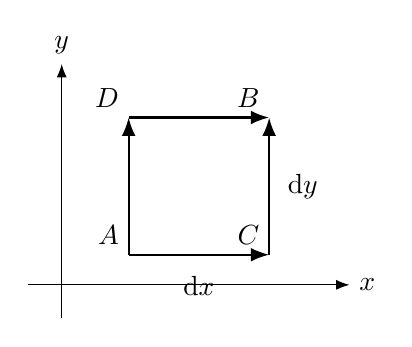
\begin{tikzpicture}[>=Latex,scale=.85]
\draw[->](-.5,0)--(4.3,0)node[right]{$x$};\draw[->](0,-.5)--(0,3.3)node[above]{$y$};
\coordinate(A)at(1,0.45);\coordinate(C)at(3.1,.45);\coordinate(D)at(1,2.5);\coordinate(B)at(3.1,2.5);
\draw[->,thick](A)--(C)node[midway,below,yshift=-4pt]{$\dd x$};\draw[->,thick](C)--(B)node[midway,right,xshift=3pt]{$\dd y$};
\draw[->,thick](A)--(D);\draw[->,thick](D)--(B);
\foreach \name in {A,B,C,D}{\node[above left]at(\name){$\name$};}
\end{tikzpicture}\end{center}
\subsection*{3) Canonical quantization}
Dirac, 1925: quantization of classical mechanical systems.

The Poisson bracket of analytical mechanics is replaced by a commutation relation in quantum mechanics:
\begin{equation}
[A,B]_{\rm P}=\sum_s\left(
\frac{\partial A}{\partial q_s}\frac{\partial B}{\partial p_s}
-\frac{\partial A}{\partial p_s}\frac{\partial B}{\partial q_s}
\right)
\longrightarrow\frac1{\ii\hbar}[\op A,\op B]
=\frac1{\ii\hbar}(\op A\op B-\op B\op A).
\end{equation}
For example,
\begin{equation}
[x_i,p_j]_{\rm P}=\delta_{ij}
\longrightarrow [\op x_i,\op p_j]=\ii\hbar\delta_{ij}.
\end{equation}
\subsection*{4) Position representation}
The matrix elements of $\op{\vect x}$ are
\begin{equation}
\mel{\vect x_1}{\op{\vect x}}{\vect x_2}
=\vect x_2\delta^{(3)}(\vect x_1-\vect x_2)
=\vect x_1\delta^{(3)}(\vect x_1-\vect x_2),
\end{equation}
so the position operator is diagonal.

From
\begin{equation}
\op U_{\mathrm{tr}}(\dd\vect x)\ket\beta
=\left(\mathbf1-\frac\ii\hbar\op{\vect p}\cdot\dd\vect x\right)\ket\beta
\end{equation}
and
\begin{equation}\begin{aligned}
\op U_{\mathrm{tr}}(\dd\vect x)\ket\beta
&=\int\dd^3x\,\ket{\vect x}\braket{\vect x-\dd\vect x}\beta\\
&=\int\dd^3x\,\ket{\vect x}\left(
\braket{\vect x}\beta-\dd\vect x\cdot\vect\nabla_{\vect x}\braket{\vect x}\beta
\right)\\
&=\ket\beta-\dd\vect x\cdot\int\dd^3x\,\ket{\vect x}\vect\nabla_{\vect x}\braket{\vect x}\beta,
\end{aligned}\end{equation}
we obtain
\begin{equation}
\op{\vect p}\ket\beta
=\int\dd^3x\,\ket{\vect x}(-\ii\hbar\vect\nabla_{\vect x})\braket{\vect x}\beta,
\end{equation}
and
\begin{equation}
\mel\alpha{\op{\vect p}}\beta
=\int\dd^3x\,\braket\alpha{\vect x}(-\ii\hbar\vect\nabla_{\vect x})\braket{\vect x}\beta.
\end{equation}
Taking $\ket\alpha=\ket{\vect x_1}$ and $\ket\beta=\ket{\vect x_2}$ gives the matrix elements of momentum in the position representation:
\begin{equation}
\mel{\vect x_1}{\op{\vect p}}{\vect x_2}
=\int\dd^3x\,\braket{\vect x_1}{\vect x}(-\ii\hbar\vect\nabla_{\vect x})\braket{\vect x}{\vect x_2}
=-\ii\hbar\vect\nabla_{\vect x_1}\delta^{(3)}(\vect x_1-\vect x_2).
\end{equation}
Now take $\ket\alpha=\ket{\vect x_1}$ and $\ket\beta=\ket{\vect p}$:
\begin{equation}
\mel{\vect x_1}{\op{\vect p}}{\vect p}
=\int\dd^3x\,\braket{\vect x_1}{\vect x}(-\ii\hbar\vect\nabla_{\vect x})\braket{\vect x}{\vect p}
=-\ii\hbar\vect\nabla_{\vect x_1}\braket{\vect x_1}{\vect p}.
\end{equation}
But the momentum eigenvalue equation gives
\begin{equation}
\vect p\braket{\vect x_1}{\vect p}
=-\ii\hbar\vect\nabla_{\vect x_1}\braket{\vect x_1}{\vect p}.
\end{equation}
Solving this first-order differential equation, we find that the momentum eigenstate in the position representation is a plane wave:
\begin{equation}
\braket{\vect x}{\vect p}=N\exp\left(\frac\ii\hbar\vect p\cdot\vect x\right).
\end{equation}
Using
\begin{equation}\begin{aligned}
\braket{\vect x_1}{\vect x_2}
&=\int\dd^3p\,\braket{\vect x_1}{\vect p}\braket{\vect p}{\vect x_2}\\
&=|N|^2\int\dd^3p\,\exp\left[\frac\ii\hbar\vect p\cdot(\vect x_1-\vect x_2)\right],
\end{aligned}\end{equation}
and
\begin{equation}
\delta^{(3)}(\vect x_1-\vect x_2)
=|N|^2(2\pi\hbar)^3\delta^{(3)}(\vect x_1-\vect x_2),
\end{equation}
we obtain
\begin{equation}
N=\frac1{(2\pi\hbar)^{3/2}},\qquad
\boxed{\braket{\vect x}{\vect p}
=\frac1{(2\pi\hbar)^{3/2}}\exp\left(\frac\ii\hbar\vect p\cdot\vect x\right).}
\end{equation}
\subsection*{5) Momentum representation}
The matrix elements of the momentum operator are
\begin{equation}
\mel{\vect p_1}{\op{\vect p}}{\vect p_2}
=\vect p_1\delta^{(3)}(\vect p_1-\vect p_2),
\end{equation}
so the momentum operator is diagonal.

For the position operator,
\begin{equation}\begin{aligned}
\mel{\vect p_1}{\op{\vect x}}{\vect p_2}
&=\int\dd^3x_1\dd^3x_2\,
\braket{\vect p_1}{\vect x_1}
\mel{\vect x_1}{\op{\vect x}}{\vect x_2}
\braket{\vect x_2}{\vect p_2}\\
&=\frac1{(2\pi\hbar)^3}\int\dd^3x_1\dd^3x_2\,
\exp\left(-\frac\ii\hbar\vect p_1\cdot\vect x_1\right)
\vect x_2\delta^{(3)}(\vect x_1-\vect x_2)
\exp\left(\frac\ii\hbar\vect p_2\cdot\vect x_2\right)\\
&=\frac1{(2\pi\hbar)^3}\int\dd^3x_1\,
\vect x_1\exp\left[\frac\ii\hbar(\vect p_2-\vect p_1)\cdot\vect x_1\right]\\
&=\ii\hbar\vect\nabla_{\vect p_1}\,
\frac1{(2\pi\hbar)^3}\int\dd^3x_1\,
\exp\left[\frac\ii\hbar(\vect p_2-\vect p_1)\cdot\vect x_1\right]\\
&=\ii\hbar\vect\nabla_{\vect p_1}\delta^{(3)}(\vect p_1-\vect p_2).
\end{aligned}\end{equation}
Note that differentiation here is with respect to momentum.

The form of the position eigenstate in the momentum representation is
\begin{equation}
\boxed{\braket{\vect p}{\vect x}
=\braket{\vect x}{\vect p}^*
=\frac1{(2\pi\hbar)^{3/2}}\exp\left(-\frac\ii\hbar\vect p\cdot\vect x\right).}
\end{equation}
\paragraph{Example 1: Prove that $\op x$ and $\op p$ are Hermitian operators in the position representation.}
For position,
\begin{equation}
\mel{x_1}{\op x}{x_2}=\delta(x_1-x_2)x_1,
\end{equation}
and
\begin{equation}\begin{aligned}
\mel{x_1}{\op x^\dagger}{x_2}
&=\mel{x_2}{\op x}{x_1}^*
=[\delta(x_2-x_1)x_2]^*
=\delta(x_2-x_1)x_2\\
&=\delta(x_1-x_2)x_1
=\mel{x_1}{\op x}{x_2}.
\end{aligned}\end{equation}
For momentum,
\begin{equation}
\mel{x_1}{\op p}{x_2}
=-\ii\hbar\frac{\partial}{\partial x_1}\delta(x_1-x_2)
=-\ii\hbar\frac{\partial}{\partial(x_1-x_2)}\delta(x_1-x_2).
\end{equation}
Also,
\begin{equation}\begin{aligned}
\mel{x_1}{\op p^\dagger}{x_2}
&=\mel{x_2}{\op p}{x_1}^*
=\left[-\ii\hbar\frac{\partial}{\partial(x_2-x_1)}\delta(x_2-x_1)\right]^*\\
&=\ii\hbar\frac{\partial}{\partial(x_2-x_1)}\delta(x_2-x_1)
=-\ii\hbar\frac{\partial}{\partial(x_1-x_2)}\delta(x_1-x_2)\\
&=\mel{x_1}{\op p}{x_2}.
\end{aligned}\end{equation}
Thus both $\op x$ and $\op p$ are Hermitian.
\paragraph{Example 2: Compute $[\op x,\op p]$ in the position representation.}
\begin{equation}\begin{aligned}
\op x\op p
&=\int\dd x_1\dd x_2\,
\op x\ket{x_1}\mel{x_1}{\op p}{x_2}\bra{x_2}\\
&=\int\dd x_1\dd x_2\,\ket{x_1}\,x_1
\left(-\ii\hbar\frac\partial{\partial x_1}\right)\delta(x_1-x_2)\bra{x_2}\\
&=-\int\dd x_1\dd x_2\,\ket{x_1}
\left(-\ii\hbar\frac\partial{\partial x_1}\right)[x_1\bra{x_1}]\,\delta(x_1-x_2)
\quad\text{(integration by parts)}\\
&=-\int\dd x_1\,\ket{x_1}
\left(-\ii\hbar\frac\partial{\partial x_1}\right)[x_1\bra{x_1}]\\
&=\int\dd x_1\,x_1\ket{x_1}
\left(-\ii\hbar\frac\partial{\partial x_1}\right)\bra{x_1}
\quad\text{(integration by parts).}
\end{aligned}\end{equation}
Similarly,
\begin{equation}
\op p\op x=-\ii\hbar+\int\dd x_1\,x_1\ket{x_1}
\left(-\ii\hbar\frac\partial{\partial x_1}\right)\bra{x_1}.
\end{equation}
Therefore
\begin{equation}
[\op x,\op p]=\ii\hbar.
\end{equation}
This shows that commutation relations do not depend on the representation.

According to the uncertainty relation, position and momentum cannot simultaneously have definite values. For example, in a momentum eigenstate the momentum has a definite value, $\mel p{(\Delta\op p)^2}p=0$, but the probability for position to take value $x$ is
\begin{equation}
|\braket x p|^2=\left|\frac1{\sqrt{2\pi\hbar}}e^{\ii px/\hbar}\right|^2
=\text{const}.
\end{equation}
The particle therefore has equal probability of appearing anywhere in $-\infty<x<\infty$; position is completely indefinite, with variance $\mel p{(\Delta\op x)^2}p=\infty$.
\paragraph{Example 3: Minimum-uncertainty wave packet.}
For equality to hold in the uncertainty relation
\begin{equation}
\langle(\Delta\op A)^2\rangle\langle(\Delta\op B)^2\rangle
\ge\left(\frac1{2\ii}\langle[\op A,\op B]\rangle\right)^2,
\end{equation}
so that the uncertainty is minimal, the state must satisfy:
\begin{enumerate}[label=\arabic*)]
\item Equality in the Schwarz inequality:
\begin{equation}
\langle(\Delta\op A)^2\rangle\langle(\Delta\op B)^2\rangle
=|\langle\Delta\op A\Delta\op B\rangle|^2.
\end{equation}
\item $\operatorname{Re}\langle\Delta\op A\Delta\op B\rangle=0$.
\end{enumerate}
The solution of condition 1 is
\begin{equation}
\Delta\op B\ket\psi=c\Delta\op A\ket\psi,
\end{equation}
where $c$ is a constant. Condition 2 implies
\begin{equation}
\operatorname{Re}\left(c\langle(\Delta\op A)^2\rangle\right)=0.
\end{equation}
Since $\langle(\Delta\op A)^2\rangle$ is real, $c=\ii a$, with $a$ real. Hence
\begin{equation}
(\op B-\langle\op B\rangle)\ket\psi
=\ii a(\op A-\langle\op A\rangle)\ket\psi.
\end{equation}
This is the constraint on $\ket\psi$ for minimum uncertainty. Choose
\begin{equation}
\op A=\op x,\qquad\op B=\op p,
\end{equation}
so
\begin{equation}
(\op p-\langle\op p\rangle)\ket\psi
=\ii a(\op x-\langle\op x\rangle)\ket\psi.
\end{equation}
In the position representation,
\begin{equation}
\left(-\ii\hbar\frac\dd{\dd x}-\langle\op p\rangle\right)\psi(x)
=\ii a(x-\langle\op x\rangle)\psi(x),\qquad
\psi(x)=\braket x\psi.
\end{equation}
The solution is
\begin{equation}
\psi(x)=A\exp\left[-\frac{a(x-\langle\op x\rangle)^2}{2\hbar}\right]
\exp\left(\frac\ii\hbar\langle\op p\rangle x\right),
\end{equation}
a Gaussian wave packet in position space.
\paragraph{Example 4: The ground state of the hydrogen atom.}
Given the state in the position representation
\begin{equation}
\braket{\vect r}\psi
=\frac1{\sqrt{\pi a_0^3}}e^{-r/a_0}\qquad\text{(hydrogen-atom ground state)},
\end{equation}
find the expectation value of the momentum.

Since $\braket{\vect r}\psi$ is not a plane wave, momentum has no definite value. The probability for momentum $\vect p$ is $|\braket{\vect p}\psi|^2$, where
\begin{equation}\begin{aligned}
\braket{\vect p}\psi
&=\int\dd^3r\,\braket{\vect p}{\vect r}\braket{\vect r}\psi
=\int\dd^3r\,\braket{\vect r}{\vect p}^*\braket{\vect r}\psi\\
&=\int\dd^3r\,\frac1{(2\pi\hbar)^{3/2}}
\exp\left(-\frac\ii\hbar\vect p\cdot\vect r\right)
\frac1{\sqrt{\pi a_0^3}}e^{-r/a_0}\\
&=\frac{(2a_0\hbar)^{3/2}\hbar}{\pi(a_0^2p^2+\hbar^2)^2}.
\end{aligned}\end{equation}
Since $\braket{\vect p}\psi$ depends only on the magnitude of momentum, the expectation value of the momentum magnitude is
\begin{equation}
\langle p\rangle=\frac{\displaystyle\int\dd p\,p^3|\braket{\vect p}\psi|^2}
{\displaystyle\int\dd p\,p^2|\braket{\vect p}\psi|^2}.
\end{equation}
\end{document}
